\section{Design}

We introduce the design framework and some implementation details.

\subsection{Overview}
In this paper, we present Z-checker, a novel framework with three important features. (1) Z-checker can be used to explore the properties of original data sets for the purpose of data analytics or improvement of lossy compression algorithms. (2) Z-checker is integrated with a rich set of evaluation algorithms and assessment functions for selecting best-fit lossy compressors for specific data sets. (3) Z-checker features both static data visualization scripts and an interactive visualization system, which can generate visual results on demand. This interactive mode allows compression algorithm developers and users to compute dynamically analysis on user-selected portions of the data set.

Z-checker is designed to support two processing modes, on-line and off-line, and two display modes, static and interactive. The four modes correspond to four different use cases. The off-line static mode is useful for generating a report on the original data set properties and the compression error, presenting multiple analysis views. The off-line interactive mode is useful for exploring the properties of the original data sets and the compression error. It allows users to dig into some region of interest and reveal local properties that are not present or visible on the whole data set. The on-line static display mode corresponds to in situ data compression and may generate and update the original data set compression analysis as long as the data is presented to Z-checker. The on-line interactive mode allows users to monitor the compression error while the data is produced. Users can zoom in on regions of interest and assess the quality of the data compression. Table \ref{tab:modes} summarizes the four use cases of Z-checker, considering the two processing modes and two visualization modes.

\begin{table}[ht] \centering
\caption{Four Use Cases of Z-checker} \centering
\scriptsize
\begin{tabular}{|l|p{0.315\columnwidth}|p{0.315\columnwidth}|}
\hline \multicolumn{1}{|c|}{} & \multicolumn{1}{|c|}{Off-line Processing}&\multicolumn{1}{|c|}{On-line Processing}\\
\hline
Static Display & Load data once for all, and view results by generating local image files. & Load data based on dynamic requests, and view results by  local image files.\\
\hline
Interactive Display & Load data once for all, and view results on demand via a web page interactively. & Load data dynamically, and view results on demand by a web page interactively. \\
\hline
\end{tabular}
\label{tab:modes}
\end{table}

 \begin{figure}[ht] \centering
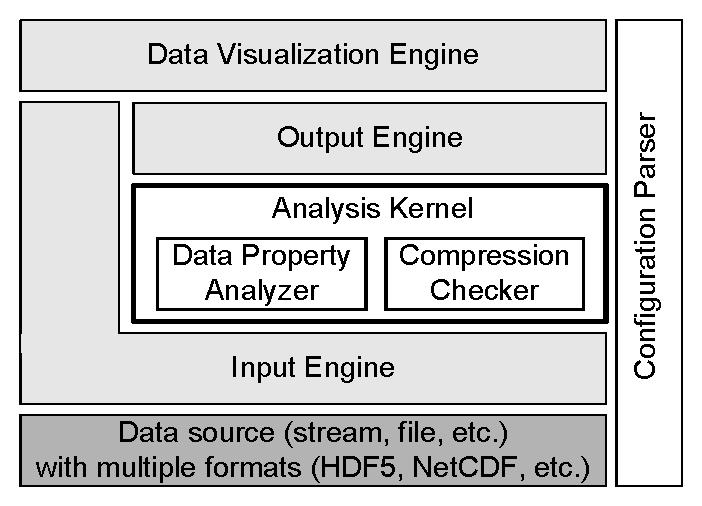
\includegraphics[scale=.6]{Figs/framework.eps}
\caption{Design Architecture of Z-checker}
\label{fig:framework}
\end{figure}

The design architecture of Z-checker is presented in Figure \ref{fig:framework}, which involves three critical parts: \emph{user interface},  \emph{processing module}, and \emph{data module}.
\begin{itemize}
\item \emph{User interface} includes three key engines---input engine, output engine, and data visualization engine---as shown in the light-gray rectangles in Figure \ref{fig:framework}. They are in charge of reading the floating-point data stream (either original data or compressed bytes), dumping the analyzed data to disks/PFS, and plotting data figures for visualizing analysis results. The Data visualization engine also provides the interactive mode through a web browser interface (details are described later).
\item \emph{Processing module}, in the whole framework, is the core module, which includes the analysis kernel and configuration parser. The former is responsible for performing the critical analysis, and the latter is in charge of parsing the user's analysis requirements (such as specifying input file path, specifying the compression command or executable, and customizing the analysis metrics on demand). Specifically, the analysis kernel is composed of two critical submodules, the data property analyzer and compression checker, which are responsible for exploring data properties based on the original data sets and analyzing the compression results with specified lossy compressors (discussed later in more detail).
\item \emph{Data source module} (shown as the dark-gray box in the figure) is the bottom layer in the whole framework and represents the data source (such as data stream produced by scientific applications at runtime or the data files stored in the disks).
\end{itemize}

\subsection{Terminology}

\begin{description}

\item[Application:] An executable program with a specific science purpose and a
designated input and output format. A given application may have multiple
executables for different target architectures and for testing different
compiler optimizations, but each such executable must have consistent
parameter, input, and output formats.

\item[Application run:] A run of an application with a given set of parameters

\item[Lossy compressors:] The library that provides lossy compression ability for scientific data sets. The science data includes different types, such as integer, single-precision and double-precision floating-point data. A lossy compressor should provide both executables and APIs for different users to call the lossy compression functions. A good lossy compressor should also provide multiple options for users to control compression errors, and it should respect the compression errors based on specified error-controlling.

\item[Compression quality:] Compression quality includes compression ratio, bit-rate, compression time, decompression time, data distortion, rate-distortion, and so on. Compression ratio is defined as the ratio of the original raw data size to the the size of the compressed data. Bit-rate refers to the number of bits used to represent one data point after the compression. Hence, bit-rate is equal to the ratio of the number of bits used by one data point originally (e.g., 64 for double-precision floating-point data) to the compression ratio. compression time and decompression time are usually evaluated by compression rate and decompression rate respectively. Compression rate is the ratio of the original raw data size (in MB) to the compression time (in seconds). The decompression rate is the ratio of the original raw data size (in MB) to the decompression time (in seconds). Data distortion involves a set of distortion metrics such as maximum compression errors, peak signal-to-noise ratio (PSNR). Rate distortion is a common metric to evaluate the compression quality. Rate, here, means the bit-rate; distortion refers to PSNR.


\item[Offline analysis:] Offline analysis means that given specific raw data files, compressed data files, and/or decompressed data files, Z-checker is able to perform the analysis and generate the report.

\item[Online analysis:] Online analysis means that Z-checker will be integrated into other tools or applications, performing the analysis with the running of applications, and generating the assessment report in the end.

\end{description}

\subsection{Dependencies}

Some functionalities of Z-checker depends on third-party libraries, which are listed as follows:

\begin{enumerate}
\item Support MPI library: ./configure --prefix=[install\_dir] --enable-mpi . (The user needs to install mpi library such as mpich before hand.)
\item Support NetCDF : usage can be found in the subdirectory NetCDFReader/ (./configure --prefix=[install\_dir] --enable-netcdf --with-netcdf-prefix=DIR; NetCDF needs to be installed in advance.)
\item Support HDF5 library: details can be found in HDF5Reader/ (./configure --prefix=[install\_dir] --enable-hdf5; the user needs to install HDF5 and set its environment variables according to HDF5 guide before hand.)
\item Support FFTW3 library: computation of 3D auto correlation requires FFTW3. In particular, 3D auto correlation is computed by using some functions provided by FFTW3. (./configure --prefix=[indall\_dir] --enable-fftw3 --with-fftw3-prefix=DIR; the user ndeeds to install FFTW3 before hand.)
\item Support R language/library: the functions coded in R script can be executed in the data analysis and compression analysis. In particular, SSIM function is coded in R, so it requires R library in Z-checker. (./configure --prefix=[index\_dir] --enable-r --with-r-prefix=DIR)
\end{enumerate}

In addition, the user can also use --with-xxx-include-path and --with-xxx-lib-path to specify the header directory and lib directory, respectively, instead of --with-xxx-prefix. More options can be found by executing "./configure -help".

\subsection{Z-checker command line format and basic usage}

\textbf{Command}: runOfflineCase\\
Description: This is a command to execute the offline analysis based on given data files and compressed/decompressed data files.
\begin{lstlisting}[style=ShellStyleInline, basicstyle = \footnotesize\ttfamily]
Usage: runOfflineCase <options>
Options:
* input information:
    -N <compressor name>: the name of the compressor
    -C <information file> : the file containing the data information
* analysis options:
    -A : perform the full analysis of the compression results
    -a <metric> : perform quick analysis for specific metric
        *metric options: (including all variables)
          cr  : compression ratio (min, avg, max)
          err : compression error (min, avg, max)
          full: complete information listed as above
* metadata options:
    -n : print number of variables
    -m : print the names of variables
    -l : list complete information of all variables
    -p : print all the precisions used in the analysis
* Examples:
    runOfflineCase -C varCmpr.inf -l
    runOfflineCase -C varCmpr.inf -m
    runOfflineCase -C varCmpr.inf -A
    runOfflineCase -C varCmpr.inf -a err
    runOfflineCase -C varCmpr.inf -a cr
\end{lstlisting}

\textbf{Command}: zccallr\\
Description: This is an executable for usrs to simply test the execution of R script files. zccallr.c is a good example to show how to call R script from C.
\begin{lstlisting}[style=ShellStyleInline, basicstyle = \footnotesize\ttfamily]
Usage: zccallr <options>
Options:
* Rscript file:
	-s <script_file>: specify the path of the R_script_file
	-c <function_name>: specify the function
* data type:
	-i : integer data (int type)
	-f : single precision (float type)
	-d : double precision (double type)
* input data files:
	-e <endian_type>: endian type of the binary data in input files:
				0(little-endian); 1(big-endian)
	-A <first data file> : first data file such as original data file
	-B <second data file> : second data file such as decompressed data file
	-C <third data file> : third data file for analysis
	-D <fourth data file> : fourth data file for analysis
	-E <fifth data file> : fifth data file for analysis
	-F <sixth data file> : sixth data file for analysis
* output type of result file:
	-r : print the result on the screen.
	-b : analysis result stored in binary format
	-t : analysis result stored in text format
	-o <output file path> : the path of the output file.
* dimensions:
	-1 <nx> : dimension for 1D data such as data[nx]
	-2 <nx> <ny> : dimensions for 2D data such as data[ny][nx]
	-3 <nx> <ny> <nz> : dimensions for 3D data such as data[nz][ny][nx]
* examples:
	zccallr -s func.R -c add1 -r -f -e 0 \
		-A ../../examples/testdata/x86/testfloat_8_8_128.dat \
				-3 8 8 128
	zccallr -s func.R -c computeErr -r -f -e 0 \
		-A ../../examples/testdata/x86/testfloat_8_8_128.dat \
		-B ../../examples/testdata/x86/testfloat_8_8_128.dat.sz.out \
		-3 8 8 128
\end{lstlisting}

\subsection{Z-checker configuration files}

1. zc.config (specifying the metrics to be used in the assessment)

This configuration file is used by many commands in Z-checker, such as analyzeDataProperty, compareDataSets.
\begin{lstlisting}[style=ShellStyleInline, basicstyle =\footnotesize\ttfamily]
#============================================================
[ENV]
#the path of the R script for special analysis such as KS_test and SSIM
#automatically set during the running of examples/Makefile
RscriptPath = /home/sdi/Z-checker/R/test/data_analysis_script.R

#endianType: either LITTLE_ENDIAN_DATA or BIG_ENDIAN_DATA
#x86, x64 and arm adopt LITTLE_ENDIAN_DATA
#PowerPC (PPC), MAC OS, and KEIL C51 adopt BIG_ENDIAN_DATA
dataEndianType = LITTLE_ENDIAN_DATA

#two statuses: either PROBE (used in detecting/monitoring compression
#results during compression) or ANALYZER (used in gleaning the results
#for plotting and analysis)
#example: checkingStatus = PROBE_COMPRESSOR
#example: checkingStatus = ANALYZE_DATA
#example: chekcingStatus = COMPARE_COMPRESSOR
checkingStatus = PROBE_COMPRESSOR

#two options for execution mode: either ONLINE or OFFLINE;
#ONLINE means running with parallel application such as MPI programs to
#check the compression at runtime (the data are produced by simulations at runtime)
#OFFLINE means running separately from the user application (the data are loaded
#from the files which are already in the disks)
executionMode = ONLINE

[DATA]
#to analyze the properties of the single data set

#compute minimal value of the data set? (1:yes, 0:no)
minValue = 1
#compute maximal value of the data set?
maxValue = 1
#value range of the data set?
valueRange = 1
#average value of the data?
avgValue = 1
#compute entrpy?
entropy = 1
#compute auto correlation of the data (to check smoothness)?
autocorr = 1
#compute 3D auto correlation of the data (to check smoothness)
autocorr3D = 1
#generate coefficients of the FFT transform?
fft = 1
#generate analysis for laplace
lap = 0

[COMPARE]
#To compare two data sets (e.g., original data vs. decompressed data)

#compression time & compression rate
compressTime = 1
#decompression time & decompression rate
decompressTime = 1
#compression size
compressSize = 1

#compute minimal absolute error between the two data sets
minAbsErr = 1
#compute average absolute error between the two data sets
avgAbsErr = 1
#compute maximal absolute error between the two data sets
maxAbsErr = 1
#compute the auto correlation of the absolute errors (white noises?)
autoCorrAbsErr = 0
#compute the 3D auto correlation of the absolute errors
autoCorrAbsErr3D = 0
#compute the PDF of the absolute errors
absErrPDF = 1
#compute the PDF of the pwr errors
pwrErrPDF = 0

#compute the value-range based minimal relative error
minRelErr = 1
#compute the value-range based average relative error
avgRelErr = 1
#compute the value-range based maximal relative error
maxRelErr = 1

#compute root mean squared error
rmse = 1
#compute normalized root mean squared error (NRMSE)
nrmse = 1
#compute peak signal-to-noise ratio (PSNR)
psnr = 1
#compute signal-to-noise ratio (SNR)
snr = 1

#compute the pearson correlation between the original data values and the
#compression errors
valErrCorr = 1

#compute the pearson correlation coefficient between the two data sets
#(to check five "nine"s?)
pearsonCorr = 1

[PLOT]
#plot the figures based on the data across different compressors or variables

#extension of property_files, which are under compressors_dir/dataProperties
propertyExtension = prop

plotAutoCorr = 1
plotFFTAmp = 1
plotEntropy = 1

plotCompressionResults = 1

plotAbsErrPDF = 1
\end{lstlisting}

2. varCmpr.info (specifying the data files to be involved in the assessment)

This configuration file is used by runOfflineCase command.
As follows, we present an example configuration file to specify a set of existing data files for assessment.
\begin{itemize}
  \item ori\_data: original data file
  \item prec: precision of the compression (such as error bound)
  \item cpr\_time: compression time (manually set by users)
  \item dec\_time: decompression time (manually set by users)
  \item cpr\_data: the path of the compressed data file
  \item dec\_data: the path of the decompressed data file
\end{itemize}
\begin{lstlisting}[style=ShellStyleInline, basicstyle =\footnotesize\ttfamily]
#information about the variables and compression demands
ori_data=CLDHGH_1_1800_3600:LITTLE_ENDIAN:FLOAT:1800x3600:../runOfflineCase_testdata/CLDHGH_1_1800_3600.dat
prec=1E-3
cpr_time=0.2
dec_time=0.1
cpr_data=../runOfflineCase_testdata/CLDHGH_1_1800_3600_1E-3.dat.sz
dec_data=../runOfflineCase_testdata/CLDHGH_1_1800_3600_1E-3.dat.sz.out
prec=1E-4
cpr_time=0.4
dec_time=0.2
cpr_data=../runOfflineCase_testdata/CLDHGH_1_1800_3600_1E-4.dat.sz
dec_data=../runOfflineCase_testdata/CLDHGH_1_1800_3600_1E-4.dat.sz.out
prec=1E-5
cpr_time=0.8
dec_time=0.4
cpr_data=../runOfflineCase_testdata/CLDHGH_1_1800_3600_1E-5.dat.sz
dec_data=../runOfflineCase_testdata/CLDHGH_1_1800_3600_1E-5.dat.sz.out
prec=1E-6
cpr_time=1.2
dec_time=0.6
cpr_data=../runOfflineCase_testdata/CLDHGH_1_1800_3600_1E-6.dat.sz
dec_data=../runOfflineCase_testdata/CLDHGH_1_1800_3600_1E-6.dat.sz.out

ori_data=CLDLOW_1_1800_3600:LITTLE_ENDIAN:FLOAT:1800x3600:../runOfflineCase_testdata/CLDLOW_1_1800_3600.dat
prec=1E-3
cpr_time=0.2
dec_time=0.1
cpr_data=../runOfflineCase_testdata/CLDLOW_1_1800_3600_1E-3.dat.sz
dec_data=../runOfflineCase_testdata/CLDLOW_1_1800_3600_1E-3.dat.sz.out
prec=1E-4
cpr_time=0.4
dec_time=0.2
cpr_data=../runOfflineCase_testdata/CLDLOW_1_1800_3600_1E-4.dat.sz
dec_data=../runOfflineCase_testdata/CLDLOW_1_1800_3600_1E-4.dat.sz.out
prec=1E-5
cpr_time=0.8
dec_time=0.4
cpr_data=../runOfflineCase_testdata/CLDLOW_1_1800_3600_1E-5.dat.sz
dec_data=../runOfflineCase_testdata/CLDLOW_1_1800_3600_1E-5.dat.sz.out
prec=1E-6
cpr_time=1.2
dec_time=0.6
cpr_data=../runOfflineCase_testdata/CLDLOW_1_1800_3600_1E-6.dat.sz
dec_data=../runOfflineCase_testdata/CLDLOW_1_1800_3600_1E-6.dat.sz.out
\end{lstlisting}

3. errBounds.cfg (specifying the error bounds used in the assessment)

This configuration is used by only One-command assessment of Z-checker-installer. Before executing the key assessment command - runZCCase.sh, the users can modify the errBounds.cfg to specify the error bounds they want to use when doing the compression/decompression test in the assessment. The runZCCase.sh will perform the compression based on the error bounds set in the errBounds.cfg and plot the compression results correspondingly.
For example, the following two lines indicate that SZ and ZFP will be used to compress the target data with four error bounds (1E-1, 1E-2, 1E-3, and 1E-4) during the assessment. 
 
SZ\_ERR\_BOUNDS = ``1E-1 1E-2 1E-3 1E-4"

ZFP\_ERR\_BOUNDS = ``1E-1 1E-2 1E-3 1E-4"

The setting comparisonCases = ``sz\_f(1E-2),sz\_d(1E-2),zfp(1E-2) sz\_f(1E-4),sz\_d(1E-4),zfp(1E-4)"  indicates that under which compressors and what error bounds the user wants to do the comparison. 
Specifically, with the above setting, the users can see the comparison results of compression ratio among the three compressors (sz\_f, sz\_d and zfp) with error bound = 1E-2 and 1E-4. 

\begin{lstlisting}[style=ShellStyleInline, basicstyle =\footnotesize\ttfamily]
#Compression error bounds for SZ
SZ_ERR_BOUNDS="1E-1 1E-2 1E-3 1E-4"

#Compression error bounds for ZFP
ZFP_ERR_BOUNDS="1E-1 1E-2 1E-3 1E-4"

#Compression cases used to compare two compressors
comparisonCases="sz_f(1E-2),sz_d(1E-2),zfp(1E-2) sz_f(1E-4),sz_d(1E-4),zfp(1E-4)"

#Number of evaluation results to be shown in the report
numOfErrorBoundCases="2"
\end{lstlisting}

\subsection{output directory layout}

\begin{lstlisting}[style=ShellStyleInline, basicstyle =\footnotesize\ttfamily]

dataProperties
    variable_1.prop         #basic property analysis results of variable 1
    variable_1.autocorr     #auto correlation of variable 1
    variable_1.lap          #lapalace results of variable 1
    variable_1.fft          #FFT transform coefficients (real and imag)
    variable_1.fft.amp      #amplitude of FFT transform
    variable_1.autocorr3d   #3D auto correlation of variable 1
    .....
    variable_N.prop         #basic property analysis results of variable N
    variable_N.autocorr     #auto correlation of variable N
    variable_N.lap          #lapalace results of variable N
    variable_N.fft          #FFT transform coefficients (real and imag)
    variable_N.fft.amp      #amplitude of FFT transform
    variable_N.autocorr3d   #3D auto correlation of variable N

compressionResults
    compressor:variable.cmp         #basic compression results
    compressor:variable.dis         #distribution of compression errors
    compressor:variable.fft         #FFT transform results of decompressed data
    compressor:variable.fft.amp     #FFT transform amplitudes of decompressed data
    compressor:variable.autocorr    #auto correlation of compression errors
    compressor:variable.autocorr3d  #3D auto correlation of compression errors
\end{lstlisting}

\subsection{One-command installation and usage}

We provide a very easy-to-use way for users to install and use Z-checker, by leveraging Z-checker-installer. In Z-checker-installer, one user can perform only one command (i.e., z-checker-install.sh) to install every related depending package or libraries, such as SZ, ZFP, gnuplot, latex. After the simple installation, the user just needs to execute two commands to finish the complete assessment procedure for a given data set. (1) Executing \emph{createZCCase.sh} can generate an individual workspace based on the user's specified test case name. (2) Executing \emph{runZCCase.sh} will perform the compression automatically by different compressors such as SZ and ZFP, and finally generate the assessment report with narratives and figures insides.
in the future, If the user wants to update his/her package based on the already installed z-checker-installer, he/she can execute one command z-checker-update.sh for simplicity, instead of rerunning z-checker-install.sh.

Both Z-checker tool and Z-checker-installer package will be put in Spack later.

\subsection{A typical test plan}

This example describes how to generate data property analysis results and compression results, given original data files (in binary), compressed files and decompressed files.

\begin{lstlisting}[style=ShellStyleInline, basicstyle =\footnotesize\ttfamily]

#Use createOfflineCase.sh to create a use-case directory, which will contain
#all the executables. Then, do the following steps.
#Preparing the testing data
.1. Download the testing data from here:
http://www.mcs.anl.gov/~shdi/download/runOfflineCase_testdata.tar.gz
#Tips: the testing data package contains two original data files and their
#corresponding SZ-compressed files and decompressed files based on different
#error bounds
.2. tar -xzvf runOfflineCase_testdata.tar.gz

#Generate the property analysis results and compression results
.3. ./createOfflineCase.sh testcase1
.4. cd testcase1
.5. ./runOfflineCase -C varCmpr.inf -A -N sz
#Tips: More options can be shown by executing ./runOfflineCase without any input
#options; in the above example, we set the compress name as "sz" because the
#compressed/decompressed data files were generated by sz.

#Generate figures based on the property/compression results in form of GNUPlot
.6. Edit zc.config as follows:
    compressors = sz:[the absolute path of the directory of the test case]
#Tips: sz here refers to the compressor name. You can replace it by your
#own compressor
    comparisonCases = sz(1E-3)
.7. ./generateGNUPlot zc.config
#Then, you can find rate-distortion eps files generated in the current directory.
#More information can be found in the doc/userguide.pdf
#Tips: You can run the executables or scripts without any inputs to see
#the help information
\end{lstlisting}

\subsection{Release Goals}
Release 0.2 for June 2018 will consist of the following functionalities.

\begin{itemize}
  \item Support both online and offline analysis
  \item Support reading of HDF5, NetCDF, Adios data
  \item One-command installation and assessment
  \item Support integration of 3rd-party libraries
  \item Z-checker web visualization
  \item Evaluation reports generated by Z-checker
\end{itemize}
